\section{Introduction}\label{sec:intro}

\begin{figure*}[t]
\centering
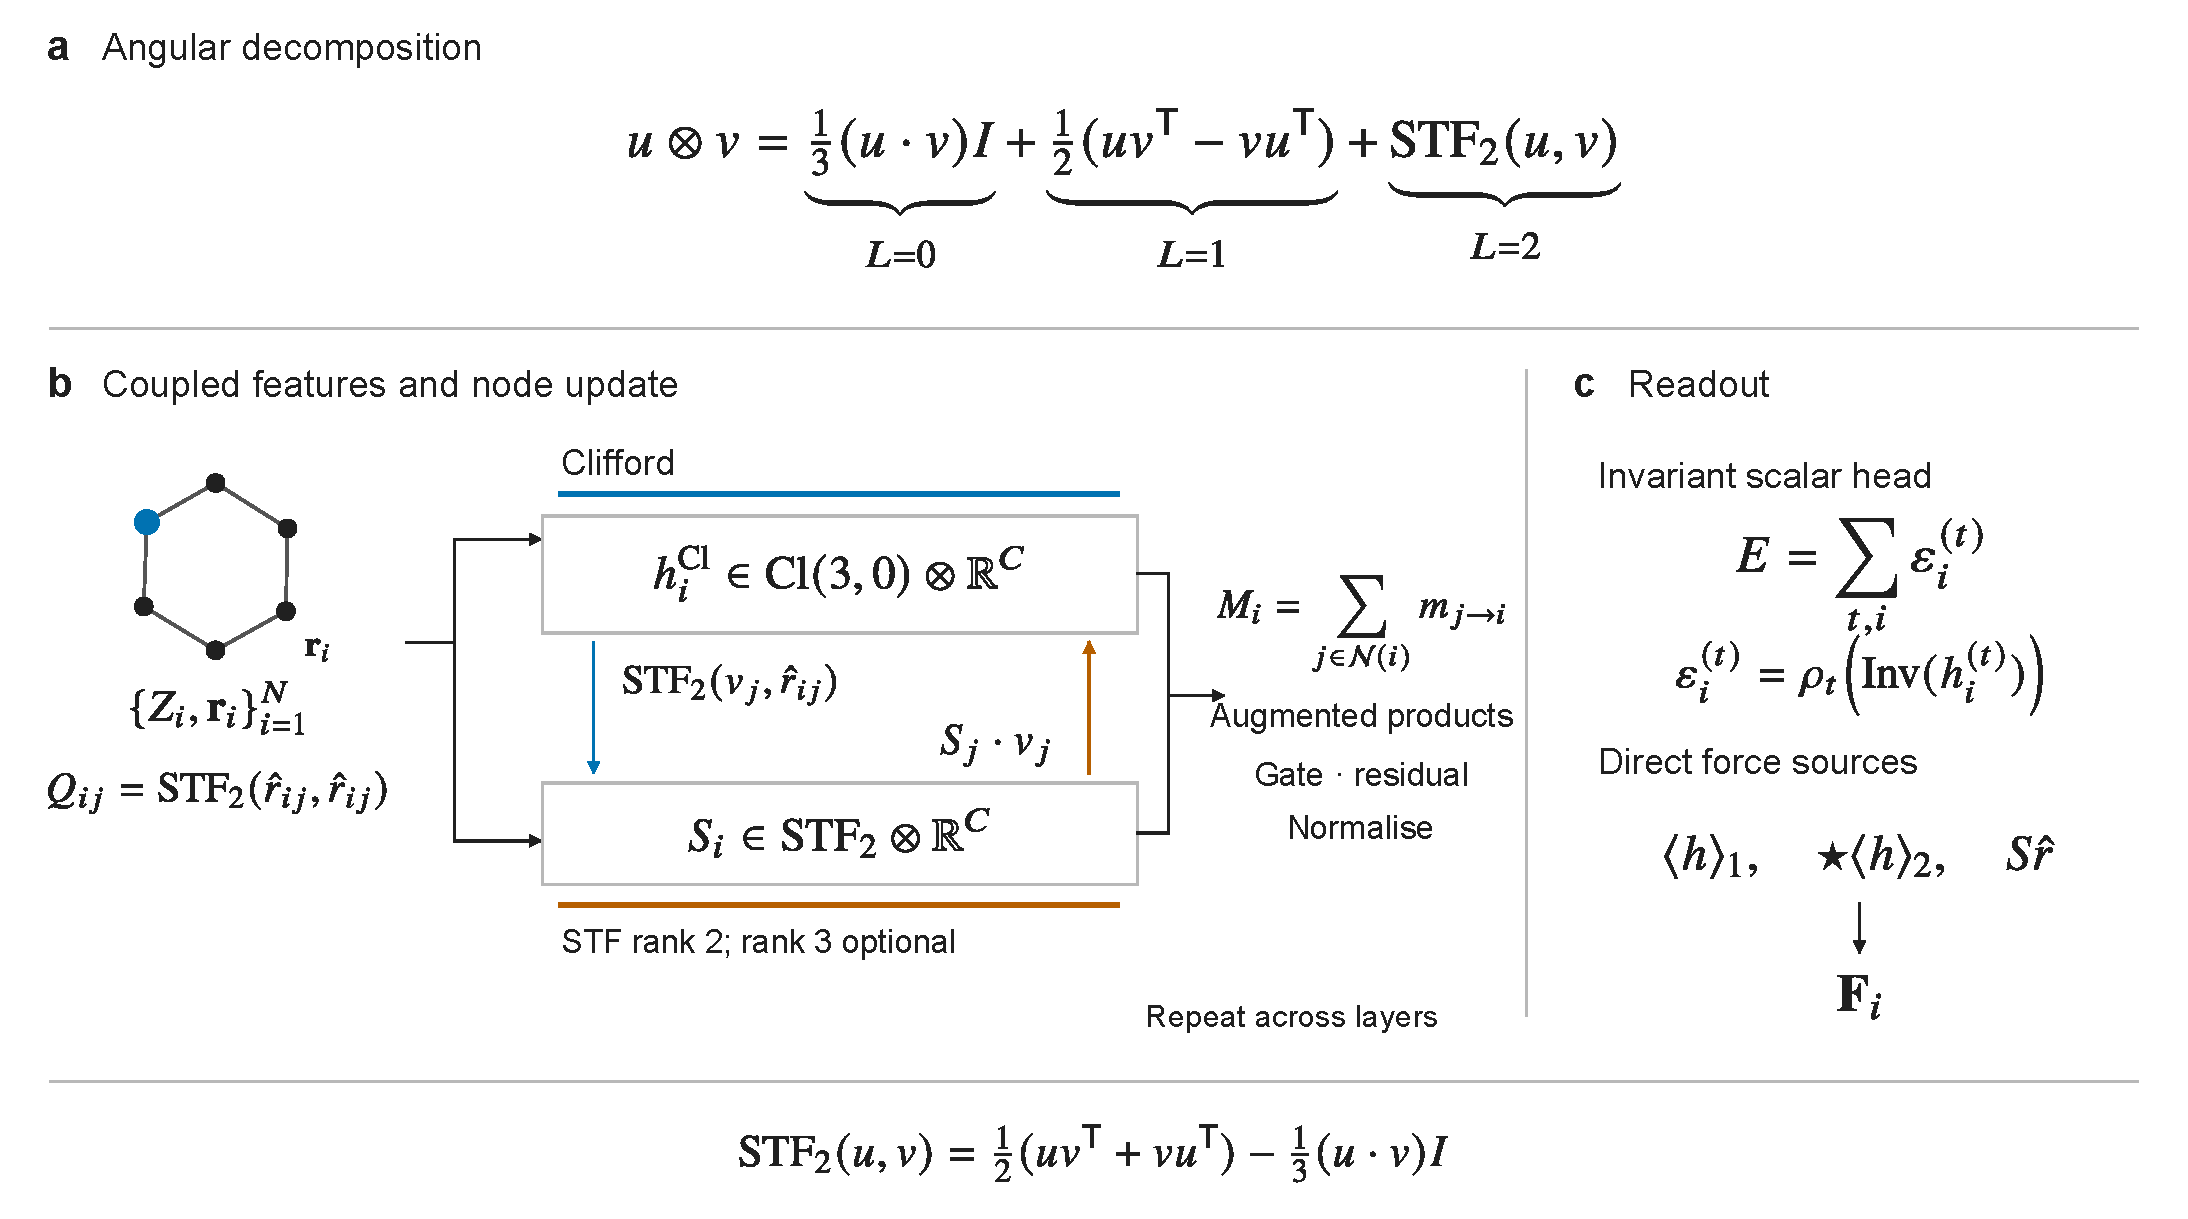
\includegraphics[width=\textwidth]{figures/fig1.pdf}
\caption{\textbf{Angular decomposition and the CliffordSTF architecture.} (a) The vector outer product separates into $L{=}0,1,2$ components (eqn~(\ref{eq:decomp})); the STF projector supplies the symmetric traceless rank-2 part \cite{simeon2023tensornet}. (b) Clifford and STF features exchange information through generation, $\mathrm{STF}_2(v_j,\hat r_{ij})$, and contraction, $S_j\cdot v_j$. Aggregated messages enter augmented products, gating, residual updates and normalisation. Here $v_j$ is the grade-1 feature, $S_j$ the rank-2 STF feature, and $C$ the channel count; rank-3 features are optional. (c) Invariant features feed the energy head, while vector, Hodge-dual and STF-contraction sources feed the direct force head.}
\label{fig:architecture}
\end{figure*}

Machine-learned interatomic potentials (MLIPs) provide practical surrogates for electronic-structure calculations, enabling molecular dynamics at scales beyond direct density functional theory \cite{unke2021machine}. The energy is invariant under rigid rotations and translations, while forces rotate with the atomic configuration and remain unchanged by translation \cite{park2021gnnff}. Force accuracy is commonly assessed through component-wise mean absolute error (MAE), but this metric does not separately identify directional agreement, and low force error alone does not establish simulation quality \cite{fu2023forces}.

Equivariant architectures commonly combine spherical-harmonic features through Clebsch--Gordan (CG) tensor products \cite{thomas2018tensor}. Cartesian alternatives perform equivariant operations directly on tensor features \cite{simeon2023tensornet,zaverkin2024ictp}. Geometric-algebra networks instead use multivectors containing scalars, vectors, oriented planes and oriented volumes, with the geometric product providing a closed-form operation for equivariant message passing \cite{ruhe2023cgenn}.

The classical vector-product decompositions distinguish the scalar and bivector output of the geometric product from the additional rank-2 symmetric traceless component of the outer product \cite{doran2003geometric,coope1965irreducible}. The latter carries angular momentum $L{=}2$, whereas the $\mathrm{Cl}(3,0)$ multivector contains only $L{=}0$ and $L{=}1$ representations \cite{lounesto2001clifford,varshalovich1988quantum}. This suggests a direct architectural question: can supplying the missing angular channels improve the forces predicted by a Clifford potential? CliffordIP \cite{polat2026cliffordip} reaches an aggregate force MAE of $0.021$\,eV\,\AA$^{-1}$ but a force cosine similarity of only $0.051$, providing a concrete setting in which to test this question.

We introduce \textbf{CliffordSTF} (Fig. \ref{fig:architecture}), which couples the Clifford multivector to symmetric traceless tensor (STF) tracks at ranks two and three through closed-form generation and contraction operations. The geometric product retains the Clifford substrate, while the STF operations introduce explicit higher-order angular features. We make three contributions:
\begin{itemize}
\item \textbf{Construction.} We combine the geometric product with classical STF projectors to recover the vector--vector CG decomposition and implement higher-order couplings through $L{=}3$, with learned maps shared across the components of each rotational representation.
\item \textbf{Mechanistic evidence.} Eleven variants plus the CliffordIP baseline isolate the role of the added features. A rank-2 edge descriptor accounts for most of the directional improvement, while the full architecture tests the additional roles of node tracks, cross-track coupling and readout.
\item \textbf{Evaluation.} CliffordSTF raises aggregate rMD17 \cite{rmd17} force cosine from $0.051$ to $0.507$ and lowers force MAE on all ten molecules. OC20 \cite{chanussot2021oc20} and OC22 \cite{tran2023oc22} test transfer to periodic systems, and larger models evaluated with energy-gradient forces demonstrate the performance attainable under longer training recipes.
\end{itemize}
